\section{課題2}
課題2のソースコードと実行結果を示す.


\subsection{課題2-1}
\lstinputlisting[caption=kadai2-1.py]{../source/kadai2-1.py}
実行結果は以下のようになった.

\begin{figure}[h]
  \begin{center}
    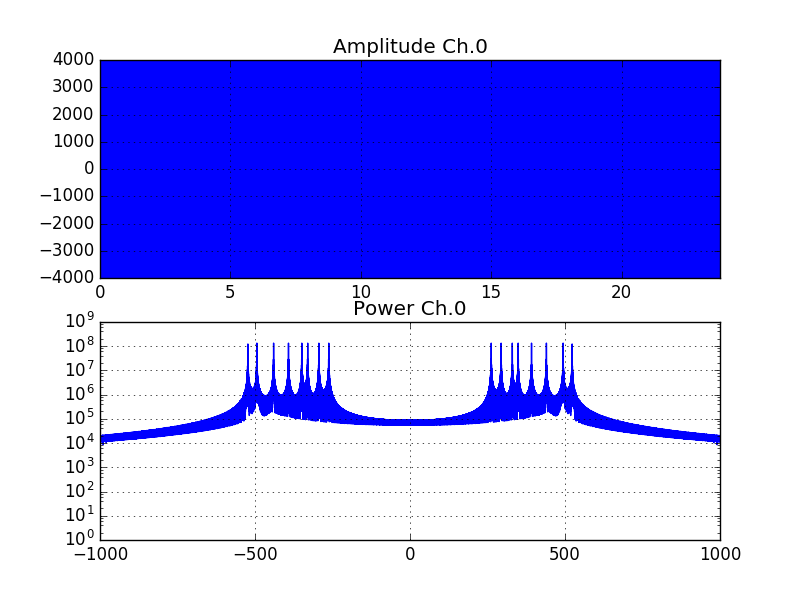
\includegraphics[width=10cm]{./img/kadai2-1.png}
    \caption{課題2-1}
  \end{center}
\end{figure}

上の波形が潰れているのは,グラフの横幅に対して波形の周波数が高すぎるためである.

下のスペクトルを確認すると262,294,330,349,393,440,494,523Hzの部分が大きく出ていることが確認できるため1オクターブ分の音声が含まれていると言える.


\subsection{課題2-2}
\lstinputlisting[caption=kadai2-2.py]{../source/kadai2-2.py}

以下,実行結果.

\begin{figure}[h]
  \begin{center}
    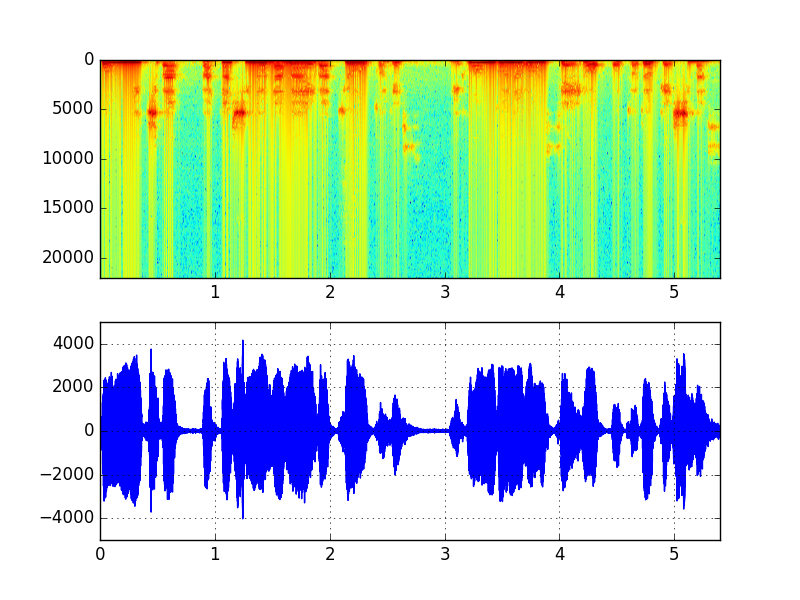
\includegraphics[width=10cm]{./img/kadai2-2.png}
    \caption{課題2-2}
  \end{center}
\end{figure}
